\documentclass[11pt,a4paper]{article}

% Marges du document %
\setlength{\topmargin}{0cm}
\setlength{\headheight}{0.4cm}
\setlength{\headsep}{0.8cm}
\setlength{\footskip}{1cm}
\setlength{\textwidth}{17cm}
\setlength{\textheight}{25cm}
\setlength{\voffset}{-1.5cm}
\setlength{\hoffset}{-0.5cm}
\setlength{\oddsidemargin}{0cm}
\setlength{\evensidemargin}{0cm}

\usepackage{amssymb}
\usepackage{psfrag}
\usepackage[utf8]{inputenc}
\usepackage[francais]{babel}
\usepackage[T1]{fontenc}
\usepackage{amsmath}
\usepackage{amsfonts}
\usepackage{amssymb}
\usepackage{graphicx}
\usepackage{subcaption}
\usepackage{fancyhdr}
\usepackage{multicol}
\usepackage{eurosym} % symbole €
\usepackage{siunitx}
\usepackage{stmaryrd}
\usepackage{bm}
\def\€{\euro{}}

\numberwithin{equation}{section}

\newcommand\numberthis{\addtocounter{equation}{1}\tag{\theequation}} 

\usepackage{color} % gestion de différentes couleurs
\definecolor{linkcolor}{rgb}{0,0,0}
\definecolor{linkcolorurl}{rgb}{0,0,1}
\usepackage[ pdftex,colorlinks=true,
pdfstartview=FitV,
linkcolor= linkcolor,
citecolor= linkcolor,
urlcolor= linkcolorurl,
hyperindex=true,
hyperfigures=false]
{hyperref} % fichiers pdf 'intelligents', avec des liens entre les références, etc.

% En-tête et pied de page % 
\pagestyle{fancy}
\fancyhead[L]{\scriptsize \textsc{Titre}} 
\fancyhead[R]{\scriptsize \textsc{BUNEL Félix et VERGNET Hadrien}} 
\fancyfoot[C]{ \thepage}

\author{Bunel Félix et Vergnet Hadrien}

%%%%%%%%%%%%%%%%%%%%%%%%%%%%%
% Tikz packages and settings
%%%%%%%%%%%%%%%%%%%%%%%%%%%%%

\usepackage{tikz}
\usepackage{pgfplots}
\usepackage{tikz-3dplot}
\pgfplotsset{compat=1.11}

\usetikzlibrary{shapes.geometric,calc,intersections}
\usetikzlibrary{shapes.arrows}
\usetikzlibrary{shadings}
\usetikzlibrary{patterns}
\usetikzlibrary{decorations.pathmorphing}
\usetikzlibrary{decorations.pathreplacing}


\usetikzlibrary{external}
\tikzset{external/aux in dpth={false}}
\tikzset{external/up to date check={simple}}
\tikzset{external/optimize command away={\includetexgraphics}{2}}

\tikzset{>=stealth}

%%%%%%%%%%%%%%%%%%%%%%%%%%%%%%%%%%%%%%%%%%%%%%%%%%%%%%%%%%%%
% Custom macro to input a tikz picture and setting its name
%%%%%%%%%%%%%%%%%%%%%%%%%%%%%%%%%%%%%%%%%%%%%%%%%%%%%%%%%%%%

\makeatletter
\newcommand{\includetikzgraphics}[1]{
	\filename@parse{#1}
	\tikzsetnextfilename{\filename@base}
	\input{#1}
}
\makeatother

%%%%%%%%%%%%%%%%%%%%%%%%%%%%%%%%%%
% Custom tikz command for drawing
%%%%%%%%%%%%%%%%%%%%%%%%%%%%%%%%%%

\tikzset{math3d/.style=
    {z= {(-0cm,-0.3cm)}, y={(0cm,1cm)},x={(1cm,0cm)}}}

% \drawYNema {x} {y} {yAngle}
\newcommand{\drawYnema}[3] {
	\shade [ball color=black] (#1,#2) ellipse 
		[x radius={sqrt(pow(cos(#3)*0.1,2)+pow(sin(#3)*0.3,2))}, y radius=0.1];
}
% \drawXNema {x} {y} {xAngle}
\newcommand{\drawXnema}[3] {
	\shade [ball color=black] (#1,#2) ellipse 
		[y radius={sqrt(pow(cos(#3)*0.1,2)+pow(sin(#3)*0.3,2))}, x radius=0.1];
}
% \drawZNema {x} {y} {zAngle}
\newcommand{\drawZnema}[3] {
	\shade [ball color=black] (#1,#2) ellipse 
		[x radius=0.3, y radius=0.1, rotate={#3}];
}

% \plotcylinder { radius } { heigth } { altitude }
\newcommand{\plotcylinder}[3] {
     \draw [math3d, fill=white, samples=100]
        plot[domain=-pi:pi] ({#1*cos(\x r)},#3,{#1*sin(\x r)}) ;
     \draw [math3d, fill=white, samples=100]
        plot[domain=0:pi] ({#1*cos(\x r)},#3,{#1*sin(\x r)}) --
        plot[domain=pi:0] ({#1*cos(\x r)},{#3-#2},{#1*sin(\x r)}) --
        cycle;
}

% \plotpolarizer { x} { y} { z } { radius } { angle }
\newcommand{\plotpolarizer}[5] {
    \draw [math3d, fill=gray, opacity=0.8, samples=100]
        plot[domain=-pi:pi] ({#1+#4*cos(\x r)},#2,{#3+#4*sin(\x r)}) ;
    \draw [math3d, opacity=0.8]
        ({#1+#4*cos(#5)},#2,{#3+#4*sin(#5)}) -- ({#1-#4*cos(#5)},#2,{#3-#4*sin(#5)}) ;
}

% \fancyarrow {xi} {yi} {xf} {yf} {width} {options}
\newcommand{\fancyarrow}[6]{
	\pgfmathsetmacro{\dx}{#3-#1};
	\pgfmathsetmacro{\dy}{#4-#2};
	\pgfmathsetmacro{\dl}{sqrt(\dx*\dx+\dy*\dy)};
	\pgfmathsetmacro{\dw}{#5/2};
	\pgfmathsetmacro{\cos}{\dx/\dl};
	\pgfmathsetmacro{\sin}{\dy/\dl};
	\draw [#6] (#1,#2) -- ++($\dw*(\sin,-\cos)$) 
		-- ++(${\dl-2*\dw}*(\cos,\sin)$)
		-- ++($\dw*(\sin,-\cos)$) -- ++($2*\dw*(\cos,\sin)+2*\dw*(-\sin,\cos)$) 
		-- ++($-2*\dw*(\cos,\sin)+2*\dw*(-\sin,\cos)$) -- ++($\dw*(\sin,-\cos)$)
		-- ++(${2*\dw-\dl}*(\cos,\sin)$) -- cycle;
}

%%%%%%%%%%%%%%%%%%%%%%%
% Custom pgf mark list
%%%%%%%%%%%%%%%%%%%%%%%
\pgfplotscreateplotcyclelist{colorhollowmarks}{%
	{black,mark=x},
	{cyan,mark=+},
	{magenta,mark=o},
	{teal,mark=square},
	{violet,mark=triangle},
	{gray,mark=diamond},
	{brown,mark=pentagon},
	{orange,mark=otimes},
	{lime,mark=10-pointed star}}
\pgfplotscreateplotcyclelist{hollowmarks}{%
	{mark=x},
	{mark=+},
	{mark=o},
	{mark=square},
	{mark=triangle},
	{mark=diamond},
	{mark=pentagona},
	{mark=otimes},
	{mark=10-pointed star}}
\pgfplotscreateplotcyclelist{onlycolors}{%
	black,
	cyan,
	magenta,
	teal,
	violet,
	lightgray,
	brown,
	orange,
	lime}



\begin{document}

%%%%%%%%%%%%%%%%%%%%%%%%%%%%%%%%%%%%%%%%%%%%%%%%%%%%%%%%%%%%%%%%%%%%%%%%%%%%%%%%%%%%%%%%
%%%%%%%%%%%%%%%%%%%%%%%%%%%%%%%%%%%%%%%%%%%%%%%%%%%%%%%%%%%%%%%%%%%%%%%%%%%%%%%%%%%%%%%%
\begin{titlepage}
%%%%%%%%%%%%%%%%%%%%%%%%%%%%%%%%%%%%%%%%%%%%%%%%%%%%%%%%%%%%%%%%%%%%%%%%%%%%%%%%%%%%%%%%
%%%%%%%%%%%%%%%%%%%%%%%%%%%%%%%%%%%%%%%%%%%%%%%%%%%%%%%%%%%%%%%%%%%%%%%%%%%%%%%%%%%%%%%%
\thispagestyle{empty}
\setlength{\parindent}{0pt}


\includegraphics[height=1.9cm]{logo-ens.jpg} \hfill 
\includegraphics[height=2cm]{logo_lyon1.jpg} \hfill 
\includegraphics[height=2cm]{logo_univ_lyon.jpg}



Master Sciences de la matière
\hfill
Projet de Transition de phase 

\textit{École Normale Supérieure de Lyon}
\hfill
BUNEL Félix et VERGNET Hadrien

\textit{Université Claude Bernard Lyon 1}
\hfill
M2 Physique 2015-2016
\vspace{0.5cm}

\hrulefill
\vspace{-0.6cm}

\hrulefill


\begin{center}\bfseries
\vspace{0.3cm}
\begin{huge}
    Exploration numérique de la transition isotrope-nématique
\end{huge}
\end{center}

\hrulefill
\vspace{-0.6cm}

\hrulefill


\begin{center}
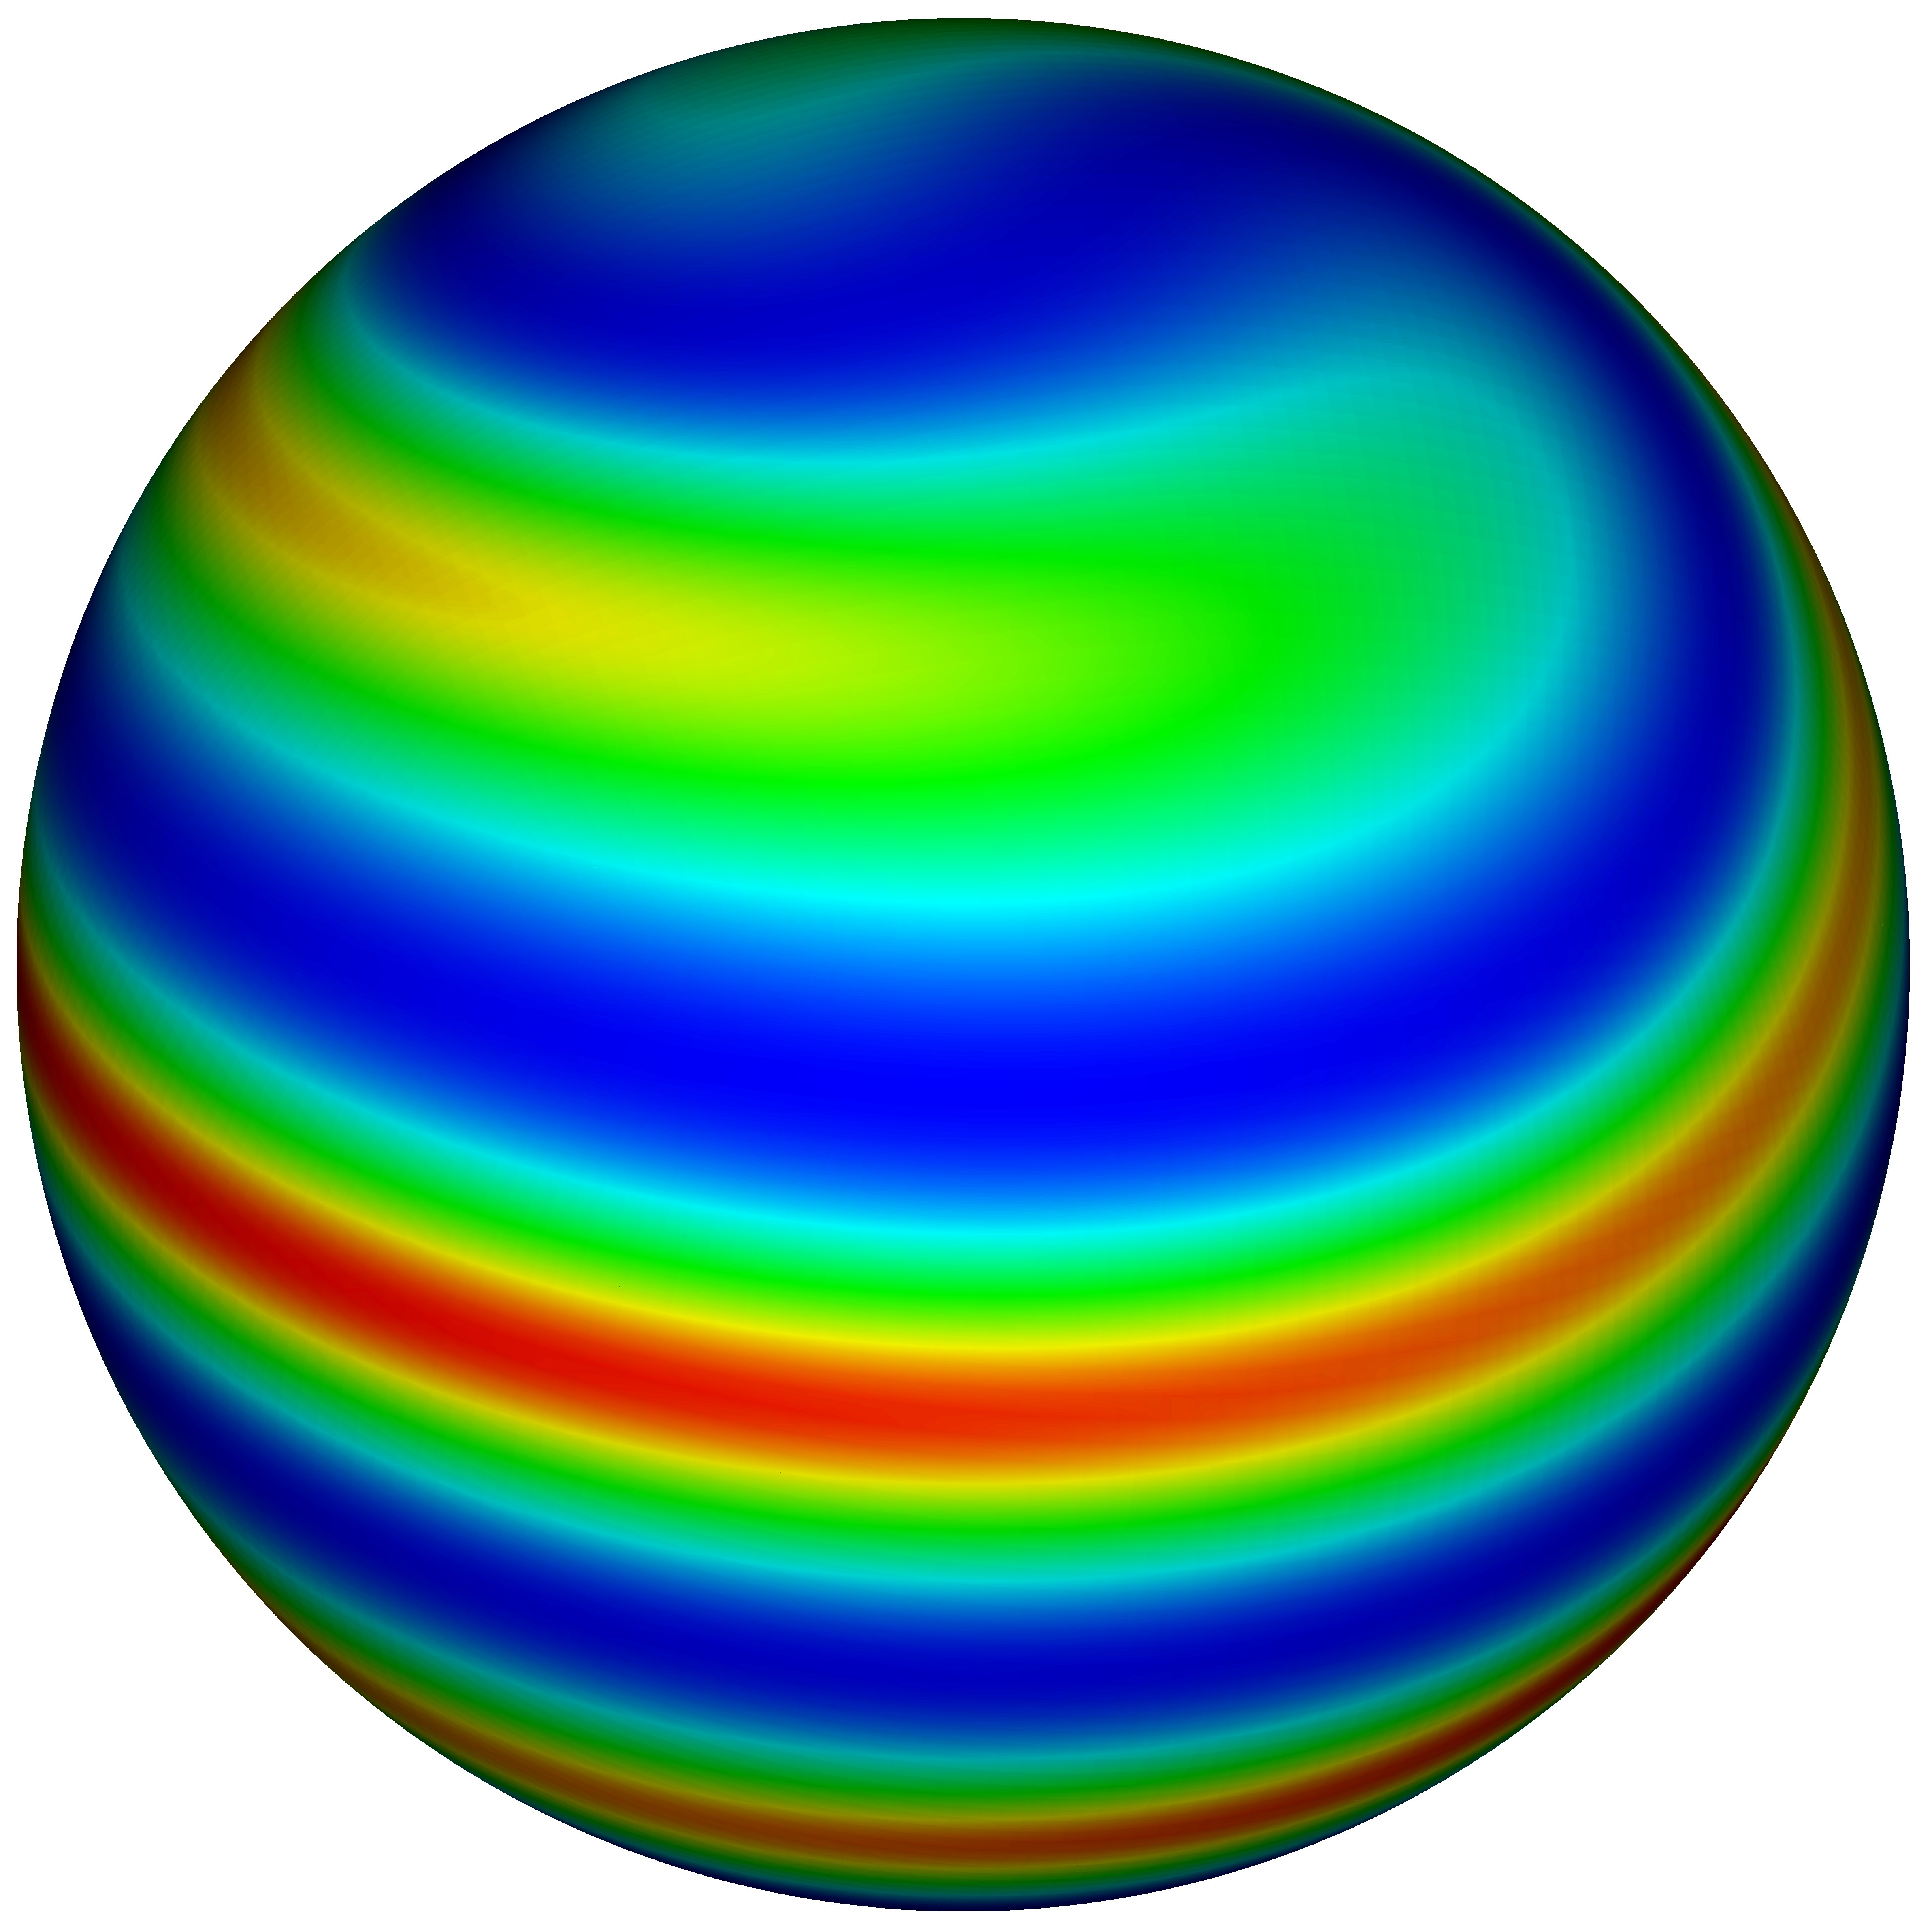
\includegraphics[height=6cm]{figures/front_simu.jpg} 
\end{center} 


\textbf{Résumé :} 
\vspace{0.3cm}

\textbf{Mots clefs :} cristaux liquides, nématique, Monte-Carlo.
\vspace{0.3cm}


\end{titlepage}

\newpage

\renewcommand\thepage{}

\section*{Remerciements}




\tableofcontents


\newpage
\renewcommand\thepage{\arabic{page}}
\setcounter{page}{1}


\definecolor{linkcolor}{rgb}{0,0,1}

%%%%%%%%%%%%%%%%%%%%%%%%%%%%%%%%%%%%%%%%%%%%%%%%%%%%%%%%%%%%%%%%%%%%%%%%%%%%%%%%%%%%%%%%
%%%%%%%%%%%%%%%%%%%%%%%%%%%%%%%%%%%%%%%%%%%%%%%%%%%%%%%%%%%%%%%%%%%%%%%%%%%%%%%%%%%%%%%%
\section*{Introduction}
%%%%%%%%%%%%%%%%%%%%%%%%%%%%%%%%%%%%%%%%%%%%%%%%%%%%%%%%%%%%%%%%%%%%%%%%%%%%%%%%%%%%%%%%
%%%%%%%%%%%%%%%%%%%%%%%%%%%%%%%%%%%%%%%%%%%%%%%%%%%%%%%%%%%%%%%%%%%%%%%%%%%%%%%%%%%%%%%%
\addcontentsline{toc}{section}{Introduction}
Le domaine des cristaux liquides a subi une importante expansion durant tout le 20\up{ème} siècle et est encore aujourd'hui un domaine actif de la recherche en physique. 
L'intérêt pour ces milieux intermédiaires entre cristaux et liquides provient entre autres de leurs applications industrielles en matière d'afficheurs (Figure \ref{lcd}).

\begin{figure}[h]
    \centering	    
	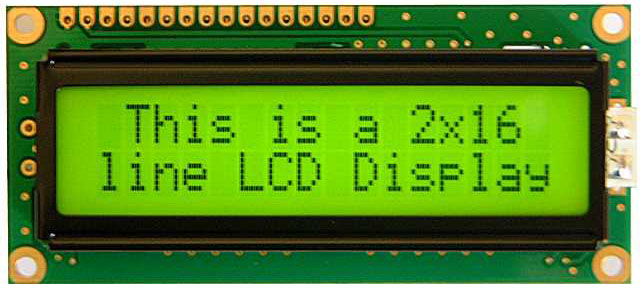
\includegraphics[height=3cm]{figures/lcd.jpg}
    \caption{Un écran à cristaux liquides}
    	\label{lcd} 
\end{figure}

Le nom cristal liquide regroupe les molécules ou mélange de molécules possédant une mésophase, à savoir une phase partiellement structurée, intermédiaire entre les phases liquide et cristalline.
Dans ce rapport, on s'intéressera au cas particulier de la phase nématique qui emprunte aux liquides l'invariance par translation, mais brise partiellement la symétrie par rotation.
Dans cette phase, les molécules s'organisent en effet pour avoir une orientation identique en moyenne (Figure \ref{nematic_phase}).

\begin{figure}[h]
    \center
    \begin{tikzpicture}[radius=0.1]
	\draw [->, >=stealth] (-1,2) -- (7.5,2) node[right]{T};
	\draw (3.35,1.9) -- (3.35,2.1) node[above]{$T^\star$};
	\draw [dashed] (3.35,2) -- (3.35,-1);

	\pgfmathsetseed{100}
	\pgfmathsetmacro{\xi}{0};
	\pgfmathsetmacro{\yi}{0};
	\foreach \i in {0,...,3}{
		\foreach \j in {0,...,2}{
			\pgfmathsetmacro{\x}{\xi+\i*0.6+0.04*rand};
			\pgfmathsetmacro{\y}{\yi+\j*0.7+0.1*rand};
			\pgfmathsetmacro{\angle}{rand*15};
			\drawZnema{\x}{\y}{\angle};
		}
	}
	\foreach \i in {0,...,3}{
		\foreach \j in {0,...,1}{
			\pgfmathsetmacro{\x}{\xi+0.3+\i*0.6+0.04*rand};
			\pgfmathsetmacro{\y}{\yi+0.35+\j*0.7+0.1*rand};
			\pgfmathsetmacro{\angle}{rand*15};
			\drawZnema{\x}{\y}{\angle};
		}
	}
	\draw [->,>=stealth] (0.5,-0.5) -- (1.5,-0.5);

	\pgfmathsetseed{79}
	\pgfmathsetmacro{\xi}{4.5};
	\pgfmathsetmacro{\yi}{0};
	\foreach \i in {0,...,3}{
		\foreach \j in {0,...,2}{
			\pgfmathsetmacro{\x}{\xi+\i*0.6+0.04*rand};
			\pgfmathsetmacro{\y}{\yi+\j*0.7+0.1*rand};
			\pgfmathsetmacro{\angle}{rand*180};
			\drawZnema{\x}{\y}{\angle};
		}
	}
	\foreach \i in {0,...,3}{
		\foreach \j in {0,...,1}{
			\pgfmathsetmacro{\x}{\xi+0.3+\i*0.6+0.04*rand};
			\pgfmathsetmacro{\y}{\yi+0.35+\j*0.7+0.1*rand};
			\pgfmathsetmacro{\angle}{rand*180};
			\drawZnema{\x}{\y}{\angle};
		}
	}


	\draw (1,-0.9) node[below]{\small phase nématique};
	\draw (5.75,-0.9) node[below]{\small phase isotrope};
\end{tikzpicture}

    \caption{Les cristaux liquides peuvent être représentées par un ensemble d'ellipsoïdes allongés dans une direction.
    Malgré les positions aléatoires des molécules, il existe un comportement collectif orientationnel : les molécules ont tendance à s'orienter dans la même direction en moyenne. }
    \label{nematic_phase}
\end{figure}

L'objectif de ce projet a été d'étudier par des méthodes numériques la transition de phase nématique-isotrope.
Ce rapport présente dans une première partie le modèle ainsi que les outils numériques utilisés. 
Une deuxième partie présentera les résultats obtenus sur la transition observée.
Enfin, une dernière partie étudiera l'influence d'un champ électrique sur cette transition.

\newpage
%%%%%%%%%%%%%%%%%%%%%%%%%%%%%%%%%%%%%%%%%%%%%%%%%%%%%%%%%%%%%%%%%%%%%%%%%%%%%%%%%%%%%%%%
%%%%%%%%%%%%%%%%%%%%%%%%%%%%%%%%%%%%%%%%%%%%%%%%%%%%%%%%%%%%%%%%%%%%%%%%%%%%%%%%%%%%%%%%
\section{Méthodes numériques}
%%%%%%%%%%%%%%%%%%%%%%%%%%%%%%%%%%%%%%%%%%%%%%%%%%%%%%%%%%%%%%%%%%%%%%%%%%%%%%%%%%%%%%%%
%%%%%%%%%%%%%%%%%%%%%%%%%%%%%%%%%%%%%%%%%%%%%%%%%%%%%%%%%%%%%%%%%%%%%%%%%%%%%%%%%%%%%%%%

\subsection{Modèle de Lebwohl-Lasher}
Le modèle de Lebwohl-Lasher \cite{model} est une version sur réseau du modèle de Maier-Saupe \cite{maier,maierbis}.
Il s'agit en quelque sorte de l'analogue pour la transition nématique-isotrope du modèle d'Ising. 
Comme le modèle d'Ising, il permet d'obtenir des résultats très satisfaisant malgré sa simplicité.
\medskip

Dans le modèle de Lebwohl-Lasher, les molécules de cristal liquides sont représentés par des vecteurs unitaires et occupent des positions fixes sur les sites d'un réseau cubique.
Les différents sites du réseau interagissent uniquement entre plus proche voisins par l'intermédiaire d'un potentiel de la forme :
\begin{equation}
E_{i,j} = - \epsilon\ \frac{3\cos^2\theta_{i,j}-1}{2}
\end{equation}
où $\epsilon$ est une constante positive et $\theta_{i,j}$ est l'angle entre les deux molécules intéressantes. 
Cette énergie est minimale lorsque les molécules sont parfaitement alignées : si $\theta_{i,j} = 0$ alors $E_{i,j} = - \epsilon$, et est maximale lorsque les molécules ont des directions orthogonales : si $\theta_{i,j} = \pi/2$ alors $E_{i,j} = \epsilon/2$.
Elle a donc tendance à favoriser les configurations ou les molécules sont alignées.
\medskip

L'énergie totale du système qui découle de cette interaction s'écrit simplement :
\begin{equation}
E_{i,j} = - \epsilon\ \sum_{<i,j>} \frac{3\cos^2\theta_{i,j}-1}{2}
\end{equation}
où $<i,j>$ est une somme sur les paires de plus voisins du réseau.

\subsection{Algorithme Monte-Carlo}


\subsection{Ratio d'acceptation}


\newpage
%%%%%%%%%%%%%%%%%%%%%%%%%%%%%%%%%%%%%%%%%%%%%%%%%%%%%%%%%%%%%%%%%%%%%%%%%%%%%%%%%%%%%%%%
%%%%%%%%%%%%%%%%%%%%%%%%%%%%%%%%%%%%%%%%%%%%%%%%%%%%%%%%%%%%%%%%%%%%%%%%%%%%%%%%%%%%%%%%
\section{Transition nématique-isotrope}
%%%%%%%%%%%%%%%%%%%%%%%%%%%%%%%%%%%%%%%%%%%%%%%%%%%%%%%%%%%%%%%%%%%%%%%%%%%%%%%%%%%%%%%%
%%%%%%%%%%%%%%%%%%%%%%%%%%%%%%%%%%%%%%%%%%%%%%%%%%%%%%%%%%%%%%%%%%%%%%%%%%%%%%%%%%%%%%%%




\newpage
%%%%%%%%%%%%%%%%%%%%%%%%%%%%%%%%%%%%%%%%%%%%%%%%%%%%%%%%%%%%%%%%%%%%%%%%%%%%%%%%%%%%%%%%
%%%%%%%%%%%%%%%%%%%%%%%%%%%%%%%%%%%%%%%%%%%%%%%%%%%%%%%%%%%%%%%%%%%%%%%%%%%%%%%%%%%%%%%%
\section{Influence d'un champ électrique}
%%%%%%%%%%%%%%%%%%%%%%%%%%%%%%%%%%%%%%%%%%%%%%%%%%%%%%%%%%%%%%%%%%%%%%%%%%%%%%%%%%%%%%%%
%%%%%%%%%%%%%%%%%%%%%%%%%%%%%%%%%%%%%%%%%%%%%%%%%%%%%%%%%%%%%%%%%%%%%%%%%%%%%%%%%%%%%%%%


\newpage
%%%%%%%%%%%%%%%%%%%%%%%%%%%%%%%%%%%%%%%%%%%%%%%%%%%%%%%%%%%%%%%%%%%%%%%%%%%%%%%%%%%%%%%%
%%%%%%%%%%%%%%%%%%%%%%%%%%%%%%%%%%%%%%%%%%%%%%%%%%%%%%%%%%%%%%%%%%%%%%%%%%%%%%%%%%%%%%%%
\section*{Conclusion}
%%%%%%%%%%%%%%%%%%%%%%%%%%%%%%%%%%%%%%%%%%%%%%%%%%%%%%%%%%%%%%%%%%%%%%%%%%%%%%%%%%%%%%%%
%%%%%%%%%%%%%%%%%%%%%%%%%%%%%%%%%%%%%%%%%%%%%%%%%%%%%%%%%%%%%%%%%%%%%%%%%%%%%%%%%%%%%%%%
\addcontentsline{toc}{section}{Conclusion}


\newpage
%%%%%%%%%%%%%%%%%%%%%%%%%%%%%%%%%%%%%%%%%%%%%%%%%%%%%%%%%%%%%%%%%%%%%%%%%%%%%%%%%%%%%%%
%%%%%%%%%%%%%%%%%%%%%%%%%%%%%%%%%%%%%%%%%%%%%%%%%%%%%%%%%%%%%%%%%%%%%%%%%%%%%%%%%%%%%%%
\appendix
%%%%%%%%%%%%%%%%%%%%%%%%%%%%%%%%%%%%%%%%%%%%%%%%%%%%%%%%%%%%%%%%%%%%%%%%%%%%%%%%%%%%%%%
%%%%%%%%%%%%%%%%%%%%%%%%%%%%%%%%%%%%%%%%%%%%%%%%%%%%%%%%%%%%%%%%%%%%%%%%%%%%%%%%%%%%%%%
\section{Première annexe} \label{annexe_fonctionnelles}


\newpage
\bibliographystyle{unsrt}
\bibliography{biblio} 
\addcontentsline{toc}{section}{Références} 


\end{document}
